\documentclass{beamer}
\usepackage[T2A]{fontenc}
\usepackage[utf8]{inputenc}
\usepackage{listings}
\usepackage{verbatim}
\usepackage{tikz}
\usetikzlibrary{shapes,arrows}

\usetheme[bullet=circle,% Use circles instead of squares for bullets.
          titleline=true,% Show a line below the frame title.
          alternativetitlepage=true,% Use the fancy title page.
          titlepagelogo=finki_logo,% Logo for the first page.
          watermark=finki_watermark,% Watermark used in every page.
          watermarkheight=50px,% Height of the watermark.
          watermarkheightmult=4,% The watermark image is 4 times bigger
                                % than watermarkheight.
          ]{FINKI2}

\author[АВ3]{М-р Ѓорѓи Маџаров\\М-р Томче Делев}
\title[Структурирано програмирање]{Аудиториски вежби 3}
\subtitle{Внес на податоци\linebreak Контролни структури за избор \texttt{if-else}}
\institute{Структурирано програмирање}
\date{Факултет за информатички науки и компјутерско инженерство - Скопје 2011}


\begin{document}

\lstset{language=C,captionpos=b,
tabsize=4,frame=lines,
basicstyle=\scriptsize\ttfamily,
keywordstyle=\color{blue},
commentstyle=\color{lightgray},
stringstyle=\color{violet},
breaklines=true,showstringspaces=false}

% Define block styles
\tikzstyle{decision} = [diamond, draw, fill=blue!20, 
    text width=4.5em, text badly centered, node distance=3cm, inner sep=0pt]
\tikzstyle{block} = [rectangle, draw, fill=blue!20, 
    text width=5em, text centered, rounded corners, minimum height=4em]
\tikzstyle{line} = [draw, -latex']
\tikzstyle{cloud} = [draw, ellipse,fill=red!20, node distance=3cm,
    minimum height=2em]

\frame[t,plain]{\titlepage}

\AtBeginSection[]
{
  \frame<handout:0>
  {
    \frametitle{Содржина}
    \tableofcontents[currentsection,hideallsubsections]
  }
}

\AtBeginSubsection[]
{
  \frame<handout:0>
  {
    \frametitle{Содржина}
    \tableofcontents[sectionstyle=show/hide,subsectionstyle=show/shaded/hide]
  }
}

% DO NOT COMPILE THIS FILE DIRECTLY!
% This is included by the other .tex files.

\section{Внес на податоци}
\begin{frame}[fragile]{RIP Dennis Ritchie}{The father of C}
\begin{center}
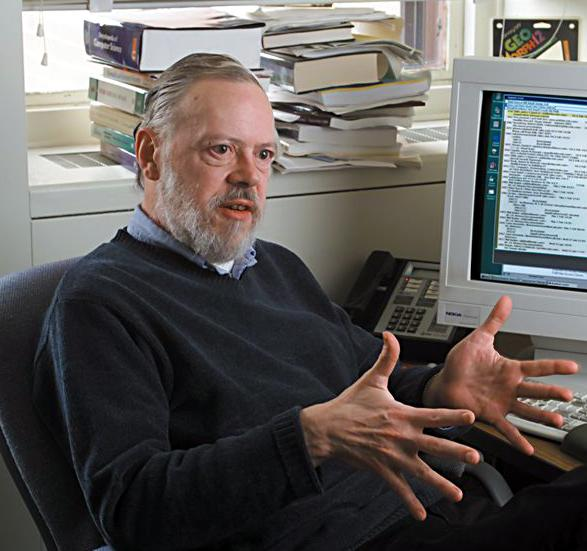
\includegraphics[scale=0.2]{images/dennis_ritchie}
\linebreak
Dennis Ritchie\\
1941 - 2011
\end{center}
\begin{lstlisting}
#include <stdio.h>
int main(void){
    printf("goodbye world :( \n");
    return(70);
}
\end{lstlisting}
\end{frame}

\begin{frame}[fragile]{Внес на податоци во C}{Функцијата \texttt{scanf}}
\begin{verbatim}
int scanf(Контролна_низа_од_знаци, arg1, arg2, ..., argn)   
\end{verbatim}  
    \begin{itemize}
    \item Контролната низа од знаци е всушност низа од знаци којa ја содржи потребната информација за форматирање   
    \item arg1, arg2, ..., argn се аргументите кои ги претставуваат индивидуалните податоци
    \end{itemize}    
\end{frame}

\begin{frame}[fragile]{Употреба на \texttt{scanf}}

\begin{exampleblock}{Пример 1}
\begin{lstlisting}
#include <stdio.h>
int main() {
    char del;
    int delbroj;
    float cena;
    scanf("%c%d%f", &del, &delbroj, &cena);
    return 0;
}
\end{lstlisting}
\end{exampleblock}
\end{frame}

\begin{frame}[fragile]{Задачa 1}
Да се напише програма за пресметување и печатење на плоштината и периметарот на круг. 
Радиусот на кругот се чита од тастатура како децимален број.
\pause
\begin{exampleblock}{Решение}
\begin{lstlisting}
#include <stdio.h>
#define PI 3.1415
int main() {
    float r;
    float P = 0, L = 0;
    printf("Vnesete go radiusot na krugot: ");
    scanf("%f", &r);
    L = 2 * r * PI;
    P = r * r * PI;
    printf("P = %f\n", P);
    printf("L = %f\n", L);
    return 0;
}
\end{lstlisting}
\end{exampleblock}
\end{frame}

\begin{frame}[fragile]{Задача 2}
Да се напише програма која чита големa буквa од тастатура и ја печати истaтa како малa буквa.\\
Помош: Секој знак се претставува со ASCII број.\\
Пр. \texttt{'А' = 65, 'а' = 97}
\pause
\begin{exampleblock}{Решение}
\begin{lstlisting}
#include <stdio.h>
int main() {
    char c;
    printf("Vnesete golema bukva: ");
    scanf("%c", &c);
    printf("%c malo se pishuva %c\n", c, c + ('a' - 'A'));
    return 0;
}
\end{lstlisting}
\end{exampleblock}
\end{frame}

\begin{frame}[fragile]{Задача 3}
Нека е дадено:
\begin{lstlisting}
    int x, y;
    y = scanf("%d", &x);
\end{lstlisting}
Каква вредност ќе има y за x=5?
\pause
    \begin{exampleblock}{Решение}
    \texttt{y = 1}
    \end{exampleblock}
\pause
Нека е дадено:
\begin{lstlisting}
    int x, y, z;
    z = scanf("%d%d", &x, &y);
\end{lstlisting}
    Каква вредност ќе има z за x=5, y=6?
\pause
    \begin{exampleblock}{Решение}
    \texttt{z = 2}
    \end{exampleblock}
\end{frame}

\begin{frame}[fragile]{Задача 4}
Да се напише програма каде од тастатура ќе се внесе цена на производ, број на рати на кои се исплаќа и 
камата (каматата е број изразен во проценти од 0 до 100). 
Програмата треба да го испечати износот на ратата и вкупната сума што ќе се исплати за производот.\\
Помош: Пресметајте ја целата сума, па потоа ратата.
\end{frame}

\begin{frame}[fragile]{Задача 4}{Решение}
    \begin{exampleblock}{Решение}
\begin{lstlisting}
#include <stdio.h>
int main() {
    float cena, kamata, rata, vkupno;
    int brRati;
    printf("Vnesete ja cenata na proizvodot: ");
    scanf("%f", &cena);
    printf("Vnesete go brojot na rati: ");
    scanf("%d", &brRati);
    printf("Vnesete ja kamata: ");
    scanf("%f", &kamata);
    vkupno = cena * (1 + kamata / 100);
    rata = vkupno / brRati;
    printf("Edna rata ke iznesuva: %.3f\n", rata);
    printf("Vkupnata isplatena suma ke bide %.3f\n",vkupno);
    return 0;
}
\end{lstlisting}
    \end{exampleblock}
\end{frame}

\begin{frame}[fragile]{Задача 5}
Да се напише програма каде од тастатура ќе се внесе трицифрен цел број. Програмата ќе ја испечати најзначајната и најмалку значајната цифра од бројот\\
Пример: Ако се внесе следниот бројот 795, програмата ќе испечати:\\
\texttt{    Najznacajna cifra e 7, a najmalku znacajna e 5.}\\
Помош: Искористете целобројно делење и остаток од делење.
\end{frame}

\begin{frame}[fragile]{Задача 5}{Решение}
    \begin{exampleblock}{Решение}
        \begin{lstlisting}
#include <stdio.h>
int main() {
    int broj;
    printf("Vnesete tricifren broj: ");
    scanf("%d", &broj);
    printf("Najznacajna cifra e %d, a najmalku znacajna e %d\n", broj / 100, broj % 10);
    return 0;
}
        \end{lstlisting}
    \end{exampleblock}
\end{frame}

\section{Контролни структури за гранење \texttt{if/else}}

\begin{frame}[fragile]{Потсетување од предавања}
\begin{center}
\begin{tikzpicture}[node distance = 2cm, auto]
    % Place nodes
    \node [decision] (decide) {Услов};
    \node [block, left of=decide, below of=decide] (true) {Наредби за точен услов};
    \node [block, right of=decide, below of=decide] (false) {Наредби за неточен услов};
    % Draw edges
    \path [line] (decide) -| node [near start] {true} (true);
    \path [line] (decide) -| node [near start] {false} (false);
\end{tikzpicture}
\begin{lstlisting}
if(uslov) {
    naredbi_za_vistinit_uslov;
} else {
    naredbi_za_nevistinit_uslov;
}
\end{lstlisting}
\end{center}
\end{frame}

\begin{frame}[fragile]{Употреба на \texttt{if}}
    \begin{exampleblock}{Пример 1}
    \begin{lstlisting}
    #include <stdio.h> 
    int main() { 
        int i;
        printf("Vnesete cel broj\n");
        scanf("%d", &i);
        if(i > 0) 
            printf("Vnesen e pozitiven broj\n");
        if(i < 0)
            printf("Vnesen e negativen broj\n"); 
        if(i == 0)
            printf("Vnesena e nula\n"); 
        return 0; 
    }
    \end{lstlisting}
    \end{exampleblock}
\end{frame}

\begin{frame}[fragile]{Со употреба на \texttt{if-else}}

    \begin{exampleblock}{Пример 2}
    \begin{lstlisting}
#include <stdio.h>
int main() {
    int i;
    printf("Vnesete cel broj\n");
    scanf("%d", &i); 
    if(i > 0)
        printf("Vnesen e pozitiven broj\n");
    else if(i < 0)
        printf("Vnesen e negativen broj\n"); 
    else
        printf("Vnesena e nula\n"); 
    return 0; 
}
    \end{lstlisting}
    \end{exampleblock}

\end{frame}

\begin{frame}[fragile]{Едноставни примери}
Што ќе отпечати?
\begin{exampleblock}{Пример 3}
    \begin{lstlisting}
#include <stdio.h>
int main() {
    int m = 5, n = 10;
    if(m > n)
        ++m;
    ++n;
    printf("m = %d, n = %d\n", m, n);
    return 0;
} 
\end{lstlisting}
\end{exampleblock}
\pause
\vfill
\texttt{m = 5, n = 11}
\end{frame}


\begin{frame}[fragile]{Задача 1}
Да се напише програма со која ќе се отпечати максимумот од два броја чии вредности се читаат од тастатура.
\pause 
    \begin{exampleblock}{Решение}
\begin{lstlisting}
#include <stdio.h>
int main() {
    int a, b;
    printf("Vnesete gi vrednostite na a i b: \n"); 
    scanf("%d %d", &a, &b);
    if(a > b)
        printf("Vrednosta na maksimumot e %d.\n", a); 
    else 
        printf("Vrednosta na maksimumot e %d.\n", b); 
    return 0; 
}
\end{lstlisting}
    \end{exampleblock}

\end{frame}

\begin{frame}[fragile]{Задача 2}
Да се напише програма која проверува дали дадена година која се вчитува од тастатура е престапна или не и на екран печати соодветна порака.\\
Пример: \texttt{1976, 2000, 2004, 2008, 2012...}
\pause
    \begin{exampleblock}{Решение}
        \begin{lstlisting}
#include <stdio.h>
int main() { 
    int godina;
    printf ("Vnesete ja godinata: \n"); 
    scanf ("%d", &godina); 
    if((godina % 4 == 0 && godina % 100 != 0) || godina % 400 == 0) 
        printf("%d godina e prestapna.\n", godina); 
    else 
        printf("%d godina ne e prestapna.\n", godina); 
    return 0; 
}
        \end{lstlisting}
    \end{exampleblock}
\end{frame}


\begin{frame}[fragile]{Задача 3}
\begin{scriptsize}
Од тастатура се внесуваат координати на една точка. Да се напише програма со која ќе се испечати на кој квадрант или оска припаѓа внесената точка. Ако станува збор за точка која лежи на координатниот почеток, да се испечати соодветна порака.
\end{scriptsize}
\pause
    \begin{exampleblock}{Решение 1 дел}
    \begin{lstlisting}
        #include <stdio.h> 
int main () { 
    float x, y;
    printf ("Vnesete kootdinati \n"); 
    scanf ("%f %f", &x, &y); 
    if(x > 0) { 
        if(y > 0) 
            printf("I Kvadrant.\n");
        else if(y < 0)
            printf("IV kvadrant.\n"); 
        else printf("Poz. x oska.\n");
        \end{lstlisting}
    \end{exampleblock}
\end{frame}



\begin{frame}[fragile]{Задача 3}{Решение}
    \begin{exampleblock}{Решение 2 дел}
        \begin{lstlisting}
         } else if(x < 0) {
        if(y > 0)
            printf("II kvadrant.\n");
        else if(y < 0) 
            printf("III kvadrant.\n");
        else
            printf("Neg. x oska.\n");
    } else {
        if(y > 0)
            printf("Poz. y oska.\n");
        else if(y < 0)
                printf("Neg. y oska.\n");
            else
                printf("Koord. pocetok\n");
    }
    return 0; 
}
        \end{lstlisting}
    \end{exampleblock}
\end{frame}



\begin{frame}[fragile]{Задача 4}
Да се напише програма која за внесен број на поени од испит ќе генерира соодветна оценка според следната табела:
\begin{center}
\begin{tabular}{|c|c|}
\hline \textbf{Поени} & \textbf{Оценка} \\ 
\hline 0 - 50 & 5 \\ 
\hline 51 - 60 & 6 \\ 
\hline 61 - 70 & 7 \\ 
\hline 71 - 80 & 8 \\ 
\hline 81 - 90 & 9 \\ 
\hline 91 - 100 & 10 \\ 
\hline
\end{tabular} 
\end{center}
\end{frame}

\begin{frame}[fragile]{Задача 4}{Решение}
\begin{exampleblock}{Решение}
        \begin{lstlisting}
        #include <stdio.h>
int main () { 
    int i, ocenka = 0;
    printf("Vnesete poeni: \n");
    scanf("%d", &i);
    if(i >= 0 && i <= 50) ocenka = 5;
    else if(i > 50 && i <= 60) ocenka = 6;
    else if(i > 60 && i <= 70) ocenka = 7;
    else if(i > 70 && i <= 80) ocenka = 8;
    else if(i > 80 && i <= 90) ocenka = 9;
    else if(i > 90 && i <= 100) ocenka = 10;
    else printf("Vnesen e pogreshen broj za poenite!!\n"); 
    if(ocenka) 
        printf("Studentot dobil ocena %d.\n", ocenka);
    return 0;
}
        \end{lstlisting}
    \end{exampleblock}
\end{frame}

\begin{frame}[fragile]{Задача 5}
Да се промени претходната програма, така што покрај оценките ќе се испечатат и знаците + и – во зависност од вредноста на последната цифра на поените:
\begin{center}
\begin{tabular}{|c|c|}
\hline \textbf{последна цифра} & \textbf{печати} \\ 
\hline 1 - 3 & - \\ 
\hline 4 - 7 & <prazno mesto> \\ 
\hline 8 - 0 & + \\ 
\hline 
\end{tabular} 
\end{center}
Пример: \texttt{81 = 9-, 94 = 10, 68 = 7+}.\\ 
За оценката 5 не треба да се додава + или –, а за оценката 10 не треба да се додава знакот +.
\end{frame}


\begin{frame}[fragile]{Задача 5}{Решение}
    \begin{exampleblock}{Решение}
        \begin{lstlisting}
        ... 
        // isto kako od prethodnata zadaca (zadaca 4)
    char znak = ' ';
    if(ocenka) {
        int p = i % 10;
        if(ocenka != 5) {
            if(p >= 1 && p <= 3) znak = '-';
                else if(ocenka != 10 && (p >= 8 || p == 0)) 
                    znak = '+';
        }
        printf("Studentot dobil ocena %d%c.\n", ocenka, znak);
    }
    return 0;
}
        \end{lstlisting}
    \end{exampleblock}
\end{frame}


\begin{frame}[fragile]{Задача 6}
Да се напише програма која ќе претставува едноставен калкулатор. Во програмата
се вчитуваат два броја и оператор во \texttt{формат}:
\begin{center}
\texttt{broj1 operator broj2}
\end{center}
По извршената операција во зависност од операторот, се печати резултатот во формат:
\begin{center}
\texttt{broj1 operator broj2 = rezultat}
\end{center}
\end{frame}

\begin{frame}[fragile,shrink=10]{Задача 6}{Решение}
    \begin{exampleblock}{Решение}
\begin{lstlisting}
#include <stdio.h>
int main() {
    char op; float br1, br2, rezultat;
    printf("Vnesete dva broja i operator vo format\n");
    printf(" broj1 operator broj2\n");
    scanf("%f %c %f", &br1, &op, &br2);
    if(op == '*') rezultat = br1 * br2;
    else if(op == '+') rezultat = br1 + br2;
    else if(op == '-') rezultat = br1 - br2;
    else if(op == '/') {
        if(br2) rezultat = br1 / br2;
        else {
            printf("Ne se deli so 0!\n");
            return 0;
        }
    } else {
        printf("Nevaliden operator!\n");
        return 0;
    }
    printf("%f %c %f = %f\n", br1, op, br2, rezultat);
    return 0;
}
        \end{lstlisting}
    \end{exampleblock}
\end{frame}


\begin{frame}[fragile]{Задача 7}
Од тастатура се внесуваат три броја кои не мора да се сортирани. Внесените броеви претставуваат должини на страните на правоаголен триаголник. Да се напише програма која што ќе проверува дали може да се конструира триаголник од дадените должини, при што ако може, треба да се провери дали истиот е правоаголен и да се пресмета неговата плоштина. Во спротивно, треба да се испечатат соодветни пораки.
\end{frame}


\begin{frame}[fragile,shrink=30]{Задача 7}{Решение}
    \begin{exampleblock}{Решение}
\begin{lstlisting}
#include <stdio.h> 
int main() {
    int a, b, c, tmp;
    printf("Vnesi gi dolzinite na stranite: \n");
    scanf("%d %d %d", &a, &b, &c);
    if((a + b <= c) || (a + c <= b) || (b + c <= a))
        printf("Ne moze da se konstruira triagolnik so tie strani.\n"a);
    else {
        if(a >= b) {
            tmp=a; a = b; b = tmp;
        }
        if(a >= c) {
            tmp = a; a = c; c = tmp;
        }
        if(b >= c) {
            tmp = b; b = c; c = tmp;
        }
        if(c * c == a * a + b * b) {
            printf("Triagolnikot e pravoagolen.\n");
            printf("Plostinata e %7.3f.\n", a * b / 2.0);
        }
        else { printf("Triagolnikot e ne pravoagolen.\n"); }
    }
    return 0;
}
        \end{lstlisting}
    \end{exampleblock}
\end{frame}

\begin{frame}{Материјали}{}
    Предавања, аудиториски вежби, соопштенија\\
    \href{http://courses.finki.ukim.mk/}{\textbf{courses.finki.ukim.mk}}
    \vfill
    Изворен код на сите примери и задачи\\
    \href{http://bitbucket.org/tdelev/finki-krs/}{\textbf{bitbucket.org/tdelev/finki-sp}}
    \vfill
    {\Huge Прашања ?}
\end{frame}
\end{document}

